\subsubsection{Subsystem Overview}
 The PLB manages the hardware-accelerated ML application, performs additional pre/post-processing on ML data (if required by the ML application), and communicates with the platform management board.

A decomposition of the system is seen in Figure \ref{pcdiag}.

Of note is the distinction between the two portions present in the PLB: the Hard Processor System (HPS) and the FPGA. The Hard Processor System is a non-customizable CPU and is used for generic tasks such as managing I/O via the Ethernet port and processing non-acceleratable ML tasks. The FPGA provides the system's \textit{programmable circuity} -- performing the requisite hardware acceleration needed for ML tasks. The two systems co-reside on the same chip, and are interfaced via internal buses.

\subsubsection{Device Selection}
The selected programmable logic board is the \textit{ZedBoard SoC Development Board} (pictured in Figure \ref{zedboard}), manufactured by Digilent. 

\begin{figure}
\centering
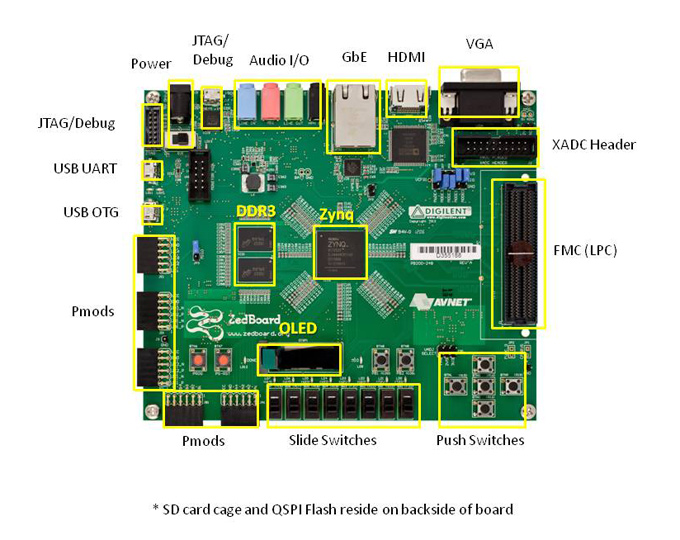
\includegraphics[width=12.5cm]{img/zedboard_functional_overview.jpg}
\caption[Layout of Connectors and Main ICs on ZedBoard]{Layout of Connectors and Main ICs on ZedBoard \cite{zedboard}}
\label{zedboard}
\end{figure}

The system specifications are as follows\cite{zedboard}:
\begin{itemize}
\item Xilinx Zynq-7000 AP SoC XC7Z020-CLG484
\item Dual-core ARM Cortex-A9 (\textit{HPS})
\item 512 MB DDR3 Random Access Memory
\item 256 MB Quad-SPI Flash Memory
\item 10/100/1000 Ethernet 
\item USB OTG 2.0 and USB-UART 
\item PS \& PL I/O expansion (FMC, Pmod, XADC)
\end{itemize}

The selection of this particular programmable logic board was mainly motivated by cost. The client was able to provide a ZedBoard unit free-of-charge, stemming from donations through the Xilinx University Program. While this board has a fairly small number of logical cells (85,000 LCs) compared to other programmable logic boards on the market, especially those which target video applications, the project's budget does not allow for the purchase of more performant boards without significant sacrifices to the multirotor assembly. The number of logical cells on the ZedBoard is sufficient to comply with the minimum LC constraint (\textbf{C.EX.1}). Additionally, the Xilinx Zynq-7000 SoC is ubiquitous in the enthusiast/academic market, providing a large amount of online resources to assist in development.

Examples of other boards examined for this project include the Nexys Artix 7 FPGA (200,000 LCs, US\$479)\cite{nexys} and the Microsemi PolarFire Video/Imaging FPGA (300,000 LCs, CAN\$1500)\cite{microsemi}. Use of the Terasic DE1-SoC (another board available free-of-charge from the client, 85,000 LCs) was also considered, but was ultimately not selected due to its poorer I/O selection and more complicated development toolchain.

\subsubsection{Data Flow}
The overall data flow managed by the PLB is as follows:
\begin{enumerate}
\item Video/ML input data is acquired by the HPS (ARM core) via the Ethernet port (from the PMB)
\item After performing any necessary clean-up/image resizing, the video frames are sent from the HPS to the FPGA via a bi-directional AXI interfaces
\item The ML IP block on the FPGA receives feature vectors (video frames) to be analyzed via the AXI buses, performs the requisite processing, and sends the results to the HPS (on the same bus)
\item The HPS interprets the results (ex. applying a sensitivity threshold) and sends these interpretations to the PMB (Raspberry Pi) via the Ethernet port
\end{enumerate}

\subsubsection{ML Hardware Accelerator Implementation}\label{ml_accel}
To facilitate the hardware acceleration of ML subtasks, a Zynq-7000-based, open-source hardware accelerator \cite{yolov2accel} (developed by graduate students at Jiangnan University) is utilized on the FPGA. As described in the accelerator's associated 2019 whitepaper\cite{yolov2unipaper}, the accelerator is capable of performing YOLOv2 \footnote{Further described in section \ref{ml_desc}} processing 112.9$\times$ faster and with 86$\times$ less power than a comparable implementation on an ARM A9 core (similar to the HPS on the Zedboard). In practice, this allows for a frame-rate (throughput) of approximately 1 FPS. As the client intends to replace this module with a custom-designed solution stemming from their research, however, this YOLOV2 accelerator is only intended as a placeholder.

At a high level, the YOLOv2 accelerator speeds up ML tasks through several optimization strategies. Most prominently, the YOLOv2 accelerator aggressively unrolls and pipelines implicit loops throughout the neural network\footnote{More information about loop unrolling can be found in Xilinx's \textit{Loop Pipelining and Loop Unrolling} guide\cite{xilinx}}. Other optimizations strategies employed include the use of 16-bit fixed point representations, parameter re-arrangement, ping-pong buffering\cite{pingpong}, and communication through parallel data buses. The module itself is written in the C language, and is converted to a hardware representation during system configuration through the use of a high-level synthesis (HLS) tool. 

In addition to the YOLOv2 accelerator, two alternative hardware acceleration units were considered for the PLB: \textit{MARLANN}\cite{marlann} and \textit{FREE-TPU}\cite{freetpu}. 

\textit{MARLANN} is an open-source IP core capable of performing 8-bit fixed point signed integer arithmetic, matrix multiplication, and max-pooling. While MARLANN has a low FPGA area overhead (approx. 5,000 LCs), its relative simplicity would necessitate a large amount of effort in developing glue logic to form a functional ML system. The MARLANN project is also not regularly maintained, leading to further concerns regarding future project maintenance/extensibility.

\textit{FREE-TPU} is a free (MIT licensed) acceleration platform developed by EmbedEEP. While the platform allows for greater flexibility in model selection compared to our selected solution (allowing for more less complex models such as MobileNet-YOLO), the project is no longer maintained. In addition, as the source code is unavailable (the API is made available as a shared library), we are prohibited from making appropriate modifications to better suit our platform (ex. modifying image data structures), leading to unacceptably poor performance (less than 0.25 FPS).

\begin{figure}[H]
\centering
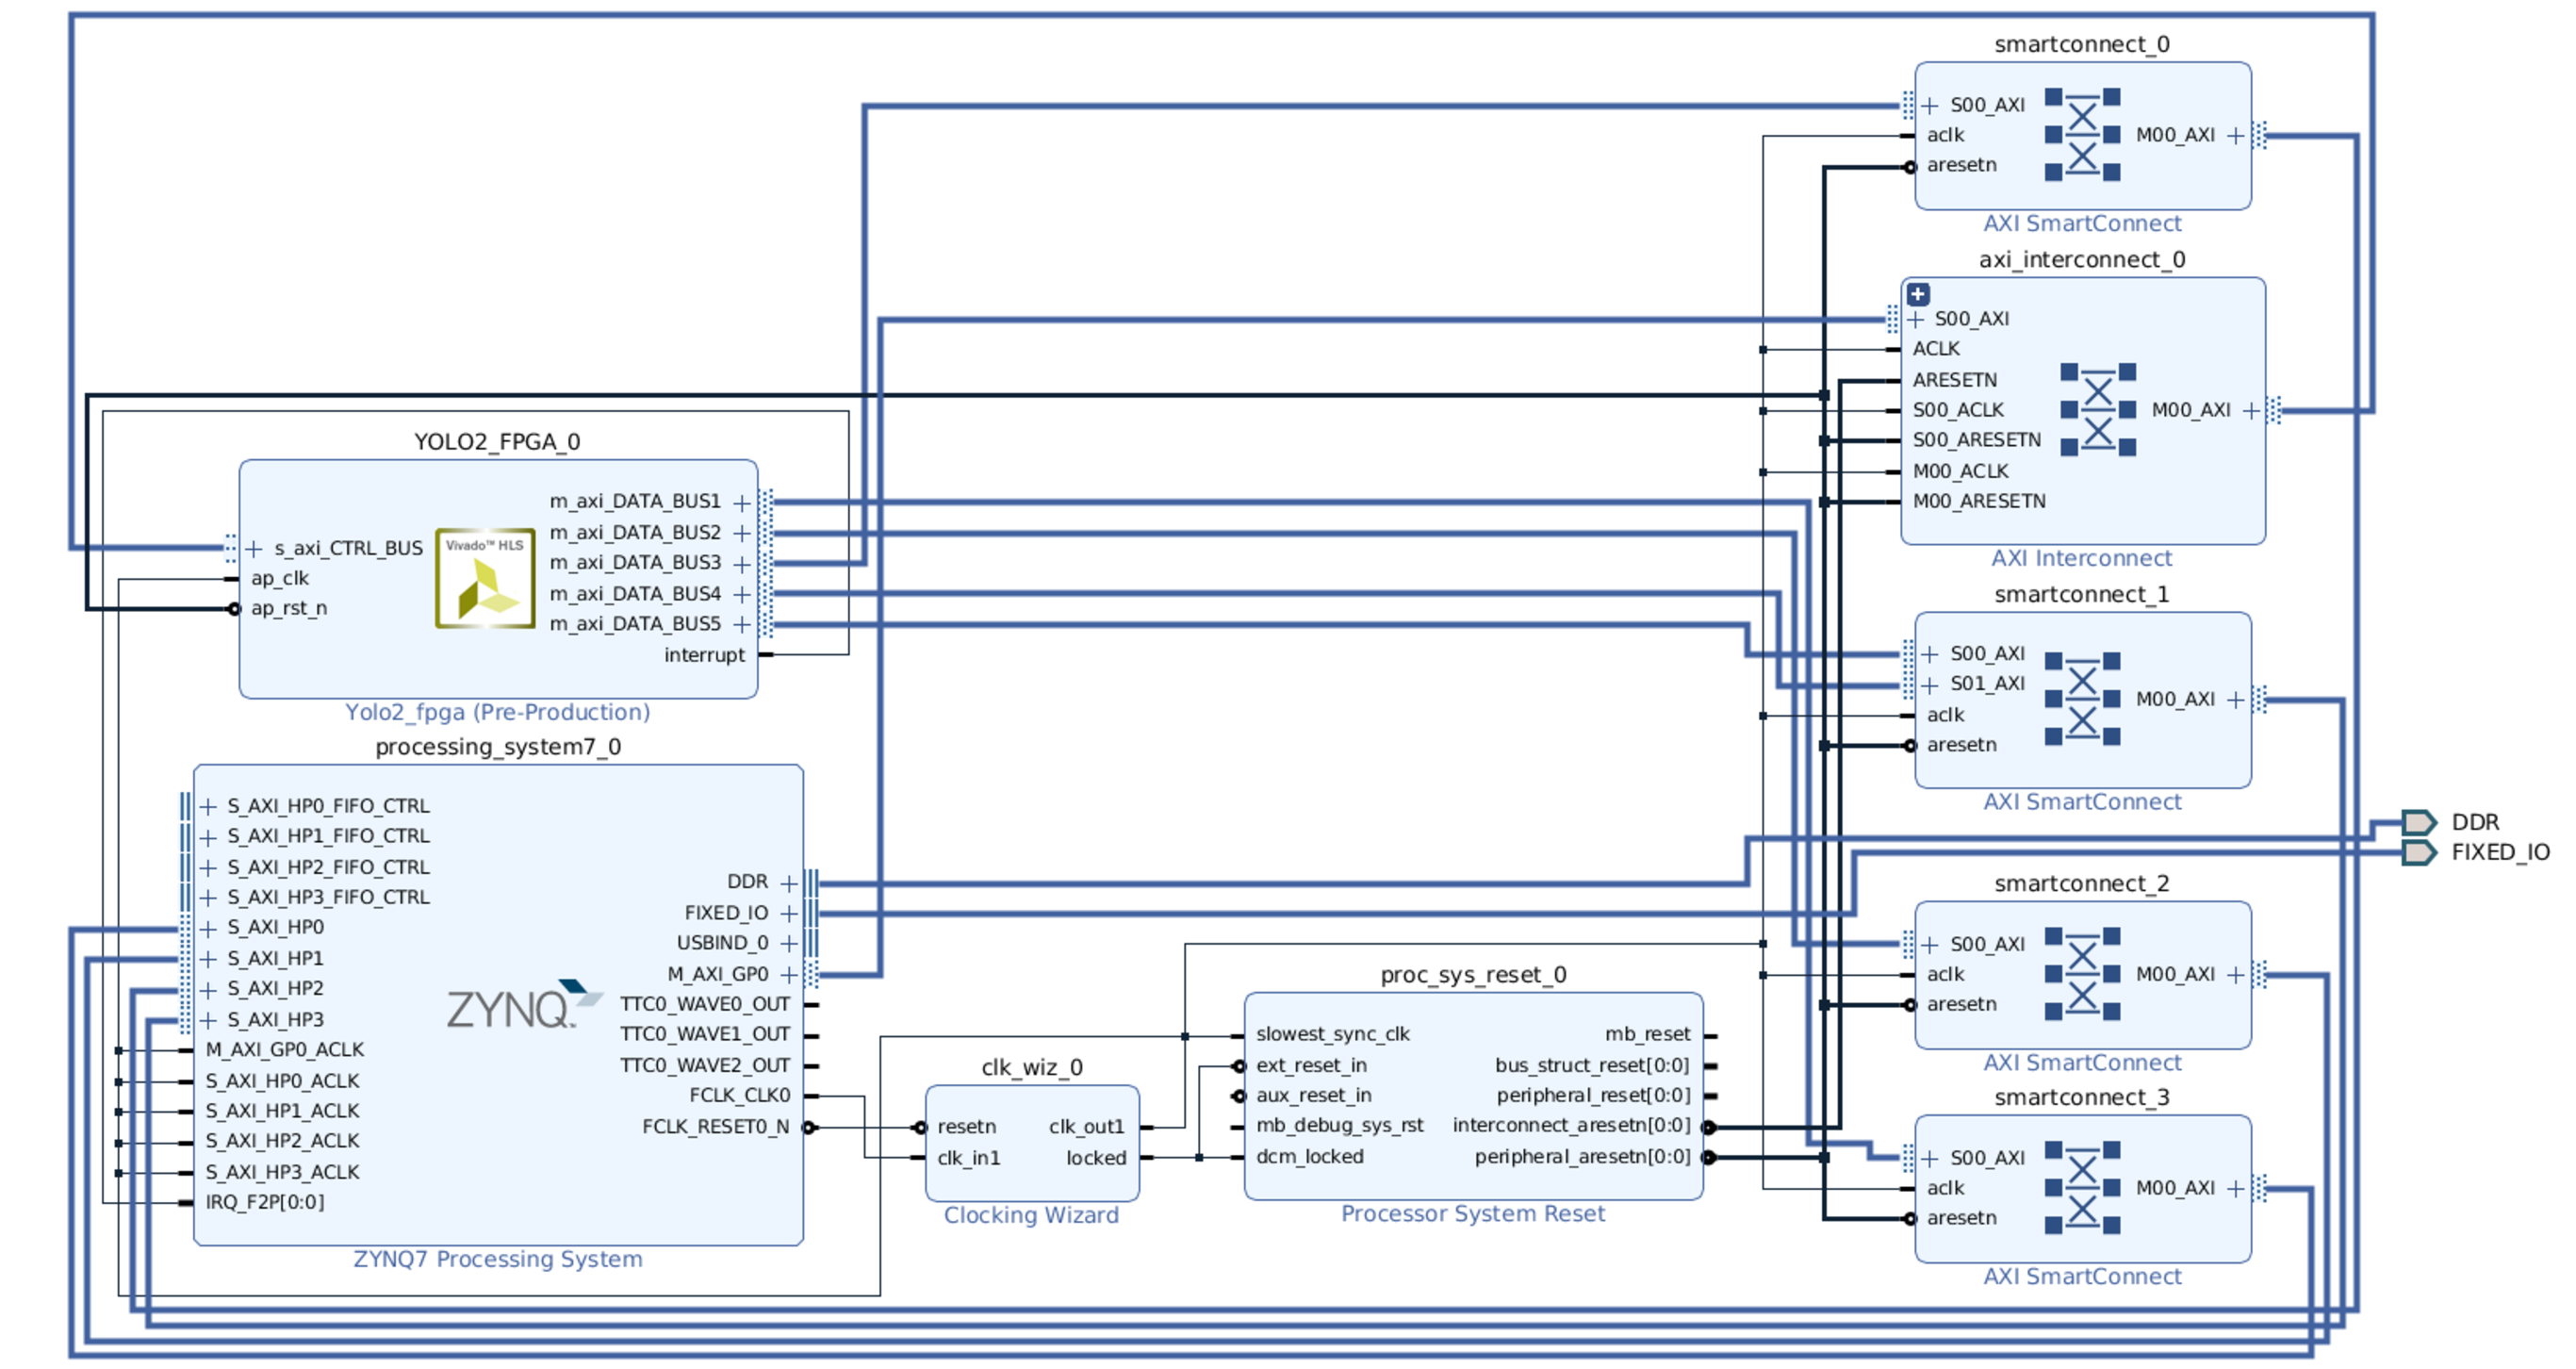
\includegraphics[width=14cm]{img/fpga_interconnect.pdf}
\caption{FPGA Interconnect Block Diagram}
\label{interconnect}
\end{figure}

\subsubsection{On-Chip Interconnects}
As seen in Figure \ref{interconnect}, the YOLOv2 accelerator is interfaced through 5 parallel AXI buses -- four buses to transfer weight data and features (including video frames) \textit{to the accelerator} and one bus to transfer system signals/results \textit{to the HPS}. A C++ program running on the HPS coordinates these interactions. In addition, each AXI bus passes through an AXI SmartConnect block (Xilinx IP) to facilitate cross-domain clocking. This is required as the YOLOv2 accelerator is driven at an higher clock frequency (150MHz compared to the provided 50MHz global clock) to further accelerate ML computations. The higher clock frequency used by the accelerator is generated through the use of a phase-locked loop (PLL) -- an efficient and commonly used construct in circuit design. The PLL is shown in Figure \ref{interconnect} as a \textit{Clocking Wizard} block.

\subsubsection{HPS Operating System}
Rather than operating on a "bare-metal" basis, a custom version of embedded Linux is used to facilitate computations and data transfer on the HPS. While an OS imposes a slight overhead, its presence greatly simplifies parallelization (required to simultaneously service requests from the PMB and acceleration core) in addition to the facilitation of debugging without the PMB attached. 

While running an existing operating system (such as Ubuntu or Raspbian) on the PLB HPS was considered, such options complicate the build and deployment of the project -- either the user must move cross-compiled helper programs onto a fresh system image, or a custom system image must be provided in the final deliverables (complicating future revisions). To alleviate these issues, Xilinx's PetaLinux development platform\cite{petalinux} is used. The PetaLinux platform automatically cross-compiles and installs helper programs into a highly-customizable Linux distribution on-the-fly. This avoids the requirement to provide compiled binaries or system images -- the user can generate (and modify) the helper programs/Linux distribution as they see fit, allowing for painless revisions.
